\section{Providing Location}

An employee's current geolocation is accessed using the
Geolocation API in the browser; to ensure the most accurate
location is returned, the \lstinline{enableHighAccuracy}
options is set.

\begin{figure}
  \centering
  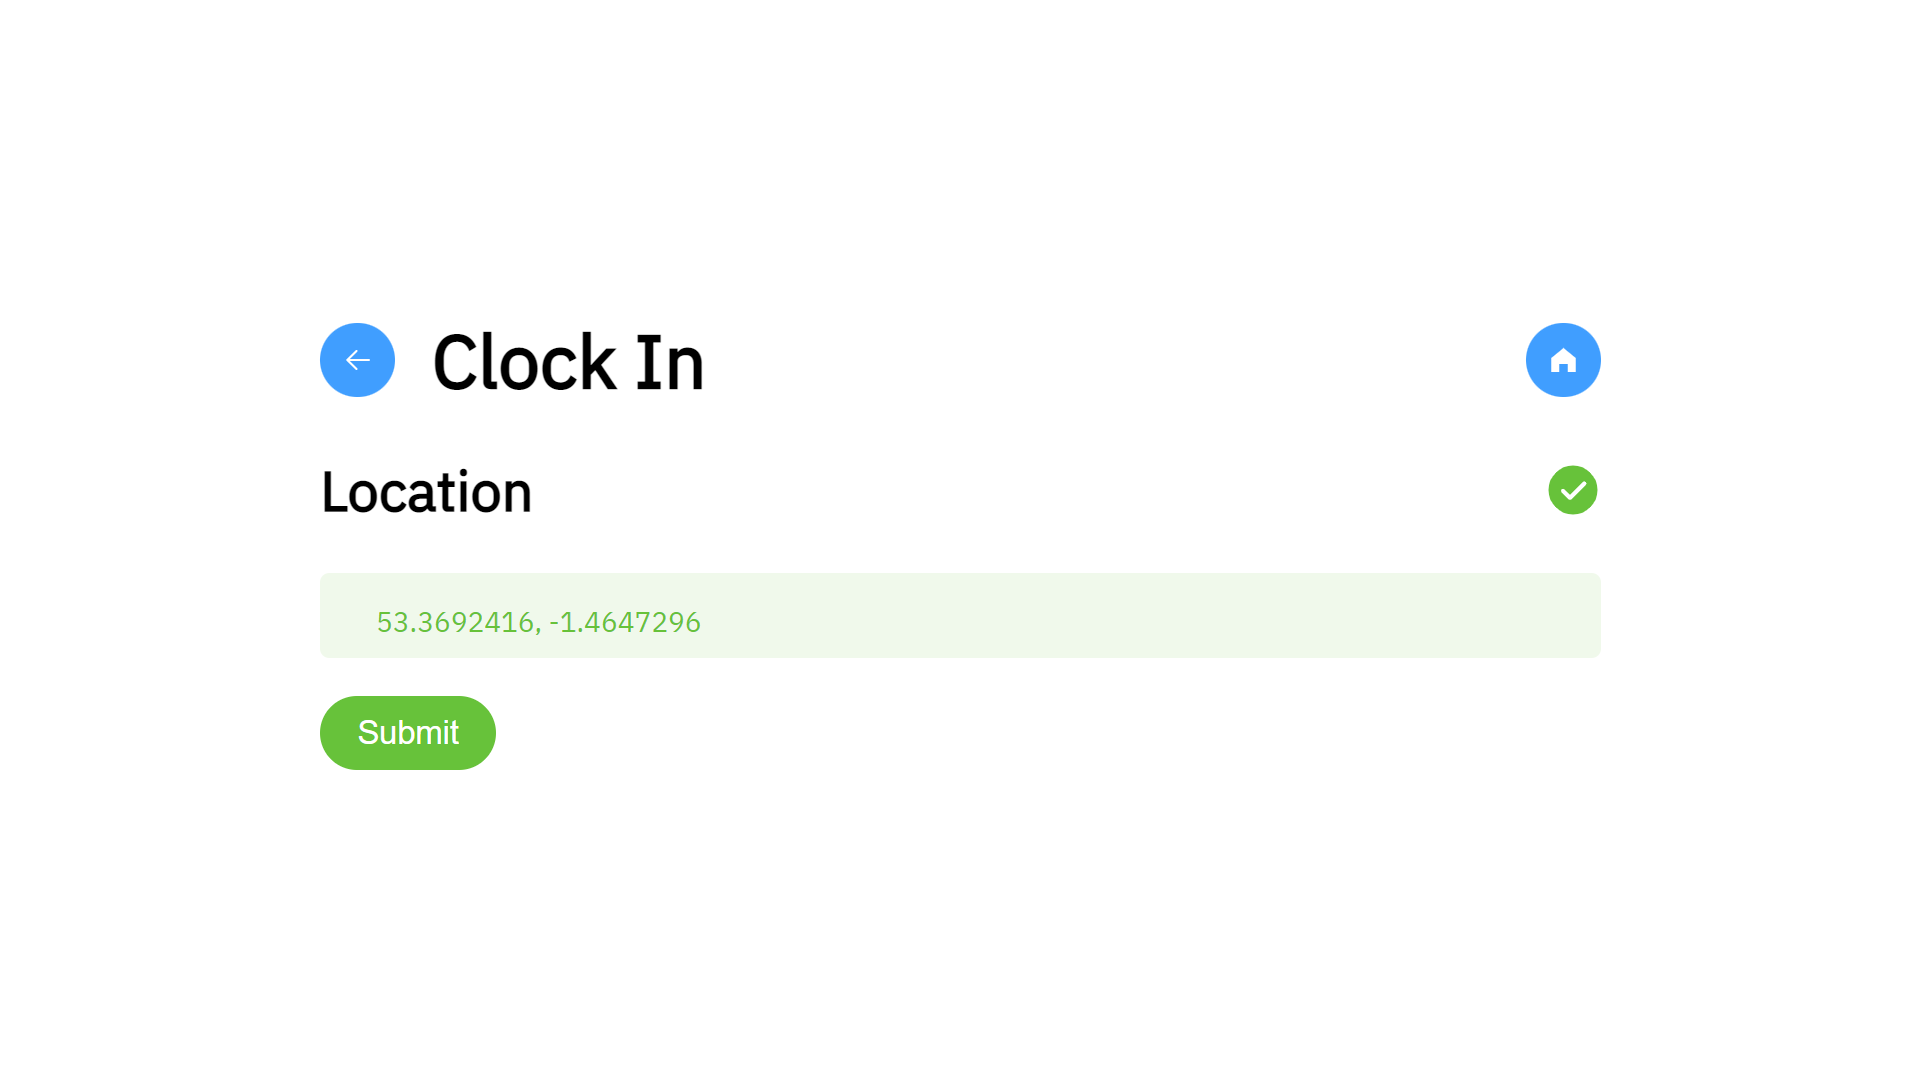
\includegraphics[width=0.8\linewidth]{06
    development/assets/providing location/clock page.png}
  \caption{Employee's location on clock in/out page}
\end{figure}

When the employee submits a clock, the backend is
responsible for measuring the distance between their
location and the job.
As noted in the \hyperref[ss:coordSystems]{research}, the
Haversine formula is the most accurate way to achieve this
with practically zero cost to performance on modern
machines.

The backend stores a latitude and longitude inside a
\lstinline{Coordinates} record, so I added a
\lstinline{Distance} method within which the formula is
implemented. 